\section{Background} \label{background}
This section describes the background of this proposal and contains information that is available but might not be known by students and readers. 

\subsection{Introduction into GUI Testing}
    Ever since the first line of software is written, testers are testing its workings. While in the early day of software, the \acrfull{ui} was mainly terminals based or a set of blinking LEDs \cite{altair8800} \footnote{For example the ALTAIR 8800 computer \cite{altair8800}}, today we have an ever-increasing amount of \acrfull{gui} applications. Testings a GUI application is labour intensive and cost a lot of money. \cite{gui-history}
    
    Initially, testers were using \acrfull{cr} software to automate their work. A tester would record a test scenario into the CR software, and then the CR software will execute the test case when needed. Using CR software, the time required to retest software decreases; however, the big downside is that when software changes, so must the recording scripts \cite{gui-history}.
    
    Then came \acrfull{mbgt}. With MBGT, the GUI elements and behaviour is abstract on a higher level. The created models are used to generate abstract test cases. Those abstract test cases need to be mapped or transformed to get concrete test cases that are executed on the SUT. The downside of MBGT is the effort required to create the models and the need to have formal modelling expertise. Formal modelling expertise is not needed with the latest next evolution in test automation: model inference. 
    
    The \emph{model inference}, also known as model extraction and GUI Ripping \cite{gui-ripping}, is the current state-of-the-art approach to automate GUI testing \cite{gui-history}. Inferred models are state graphs based on the GUI of the SUT. There are two ways to generate inferred models; the first is a static approach where the source code of the  SUT is used to create a GUI model. The second is a dynamic approach where the GUI state is captured and extracted while being executed. 
    
    The static approach has several downsides. First, the source code must be available, which is not always the case and secondly, it is challenging to capture behaviour based on the GUI source code. For example, with HTML, it is easy to generate a model; however, its behaviour is either in Javascript or server code.  It is possible to overcome those stumbling blocks by executing the SUT.
    
    As for the Dynamic approach, it captures the model during test execution. The automated test tool interacts with the SUT in a scriptless and random way. This random scriptless approach is called \emph{Monkey testing}. Usually, test monkeys have no idea in which state the SUT is in and what type of input is allowed. It is therefore essential to make the test monkey smarter. A "smart test monkey" can be achieved by making them "see" the UI elements (Section \ref{data-retrieval}). Section \ref{testar-testauto} will give more details about how TESTAR is using smart test monkeys.

\subsection{What is TESTAR?} \label{what-is-testar}
TESTAR - or TEST* - is an automated software testing tool for the GUI level \cite{testar-about}. TESTAR started within the context of the \acrfull{fittest} project. TESTAR is open-source, the source code is published on GitHub \footnote{ \url{https://github.com/TESTARtool/TESTAR\_dev}}. A screenshot of the TESTAR tool is displayed in Figure \ref{fig:testar}.

\begingroup
\captionsetup{type=figure}
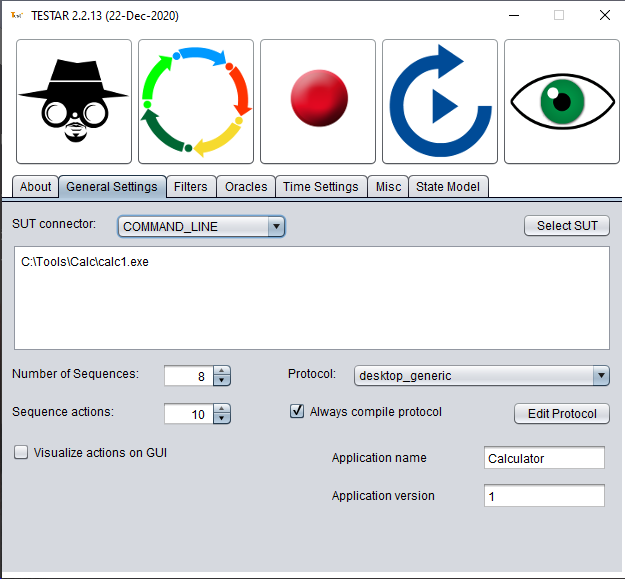
\includegraphics[scale=0.5]{pics/testar.png}
\captionof{figure}{Screenshot of the TESTAR tool}\label{fig:testar}
\endgroup

TESTAR has several \emph{execution modes} in which it interacts with the SUT \cite{testar-manual}. From left to right, in figure \ref{fig:testar}, those are Spy, Generate, Record, Replay and View mode. 

The \emph{Spy} mode allows the user to inspect a SUT and analyse how TESTAR is interpreting the widgets on the screen. Figure \ref{fig:calc-spy} shows the Windows calculator in spy mode. Dots on the GUI indicates actions with which TESTAR can interact. Furthermore, within TESTAR, it is possible to filter out actions. TESTAR will then not execute those actions. The actions are marked with a silver-coloured dot. A list with properties about the widget is shown when hovering, as well as a unique identifier of the current \emph{state}, more information about the state and the unique identifier can be found at section \ref{gui-state}.\par

\begingroup
\captionsetup{type=figure}
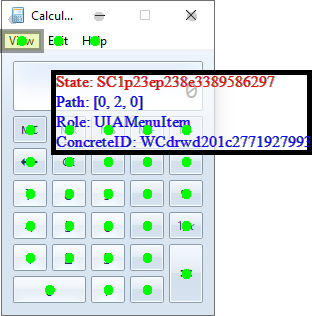
\includegraphics{pics/calc-state.png}
\captionof{figure}{Screenshot of the Calculator with TESTAR Spy}\label{fig:calc-spy}
\endgroup

In the \emph{Generate} mode, TESTAR will start testing the specified system. Section \ref{testar-testauto} gives for more details about TESTAR test automation.

The \emph{Record} mode allows a tester to record a test sequence manually. In the \emph{Replay} mode, existing test execution can be re-executed and lastly, the \emph{Review} mode allows existing test executions to be viewed.

\subsubsection{TEST automation} \label{testar-testauto}
TESTAR works without any test scripts but is uses GUI Ripper and Monkey testing techniques. \emph{GUI Ripping}, first introduced by Memon et al. \cite{gui-ripping} and is a process to obtain the GUI's structure and execution behaviour automatically. As for \emph{Monkey testing}, it is a process in which decisions (interactions with the GUI) are randomly made. Section \ref{data-retrieval} will give more insights into GUI Ripping.
TESTAR is using a flow to execute tests on the SUT. This flow is as follows:
\begin{enumerate}
    \item Start the SUT
    \item Scan the GUI and obtain the state (Section \ref{gui-state})
    \item Finding and selecting an action to execute
    \item Evaluate state with a test oracle (Section \ref{test-oracles})
    \item Stop the SUT when no actions are left to be executed or restart the SUT when more sequences are required.
\end{enumerate}

\begingroup
\captionsetup{type=figure}
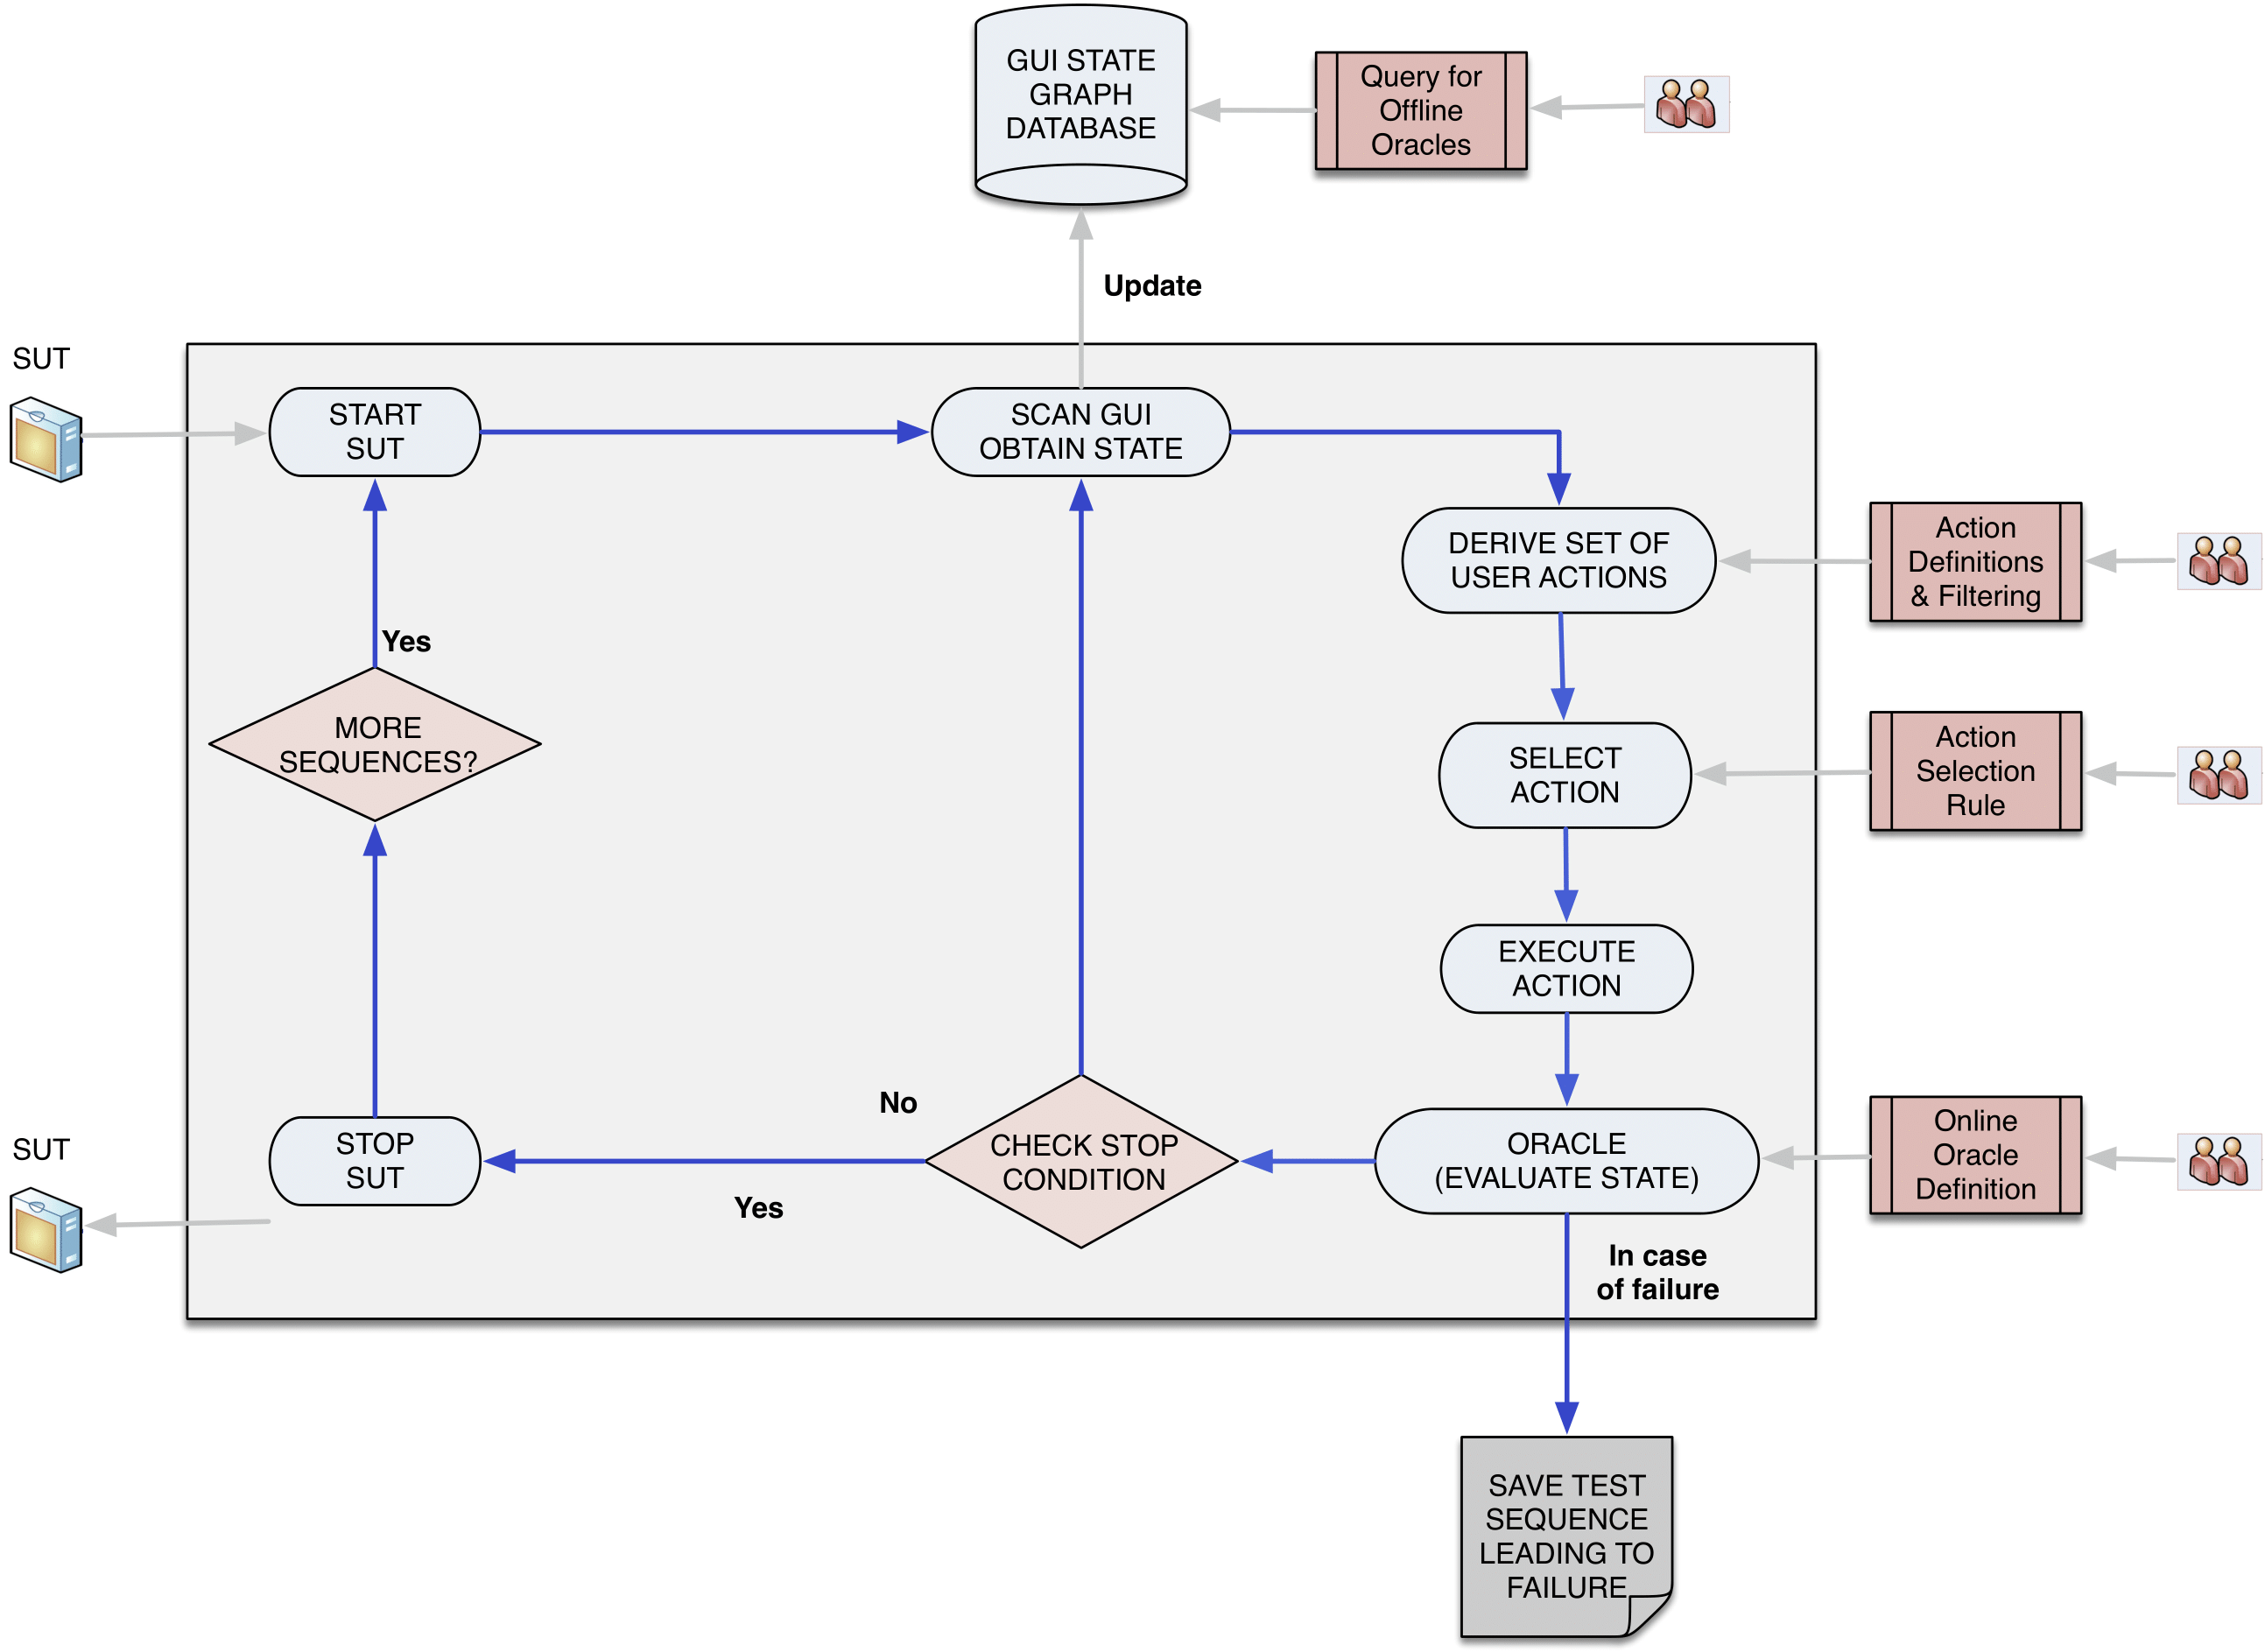
\includegraphics[scale=0.8]{pics/testar-test-cycle.png}
\captionof{figure}{TESTAR test cycle \cite{VosAho2021}}\label{fig:testar-test-cycle}
\endgroup

Figure \ref{fig:testar-test-cycle} shows the flow graphically \cite{VosAho2021}. The test specialist needs to provide SUT details to TESTAR, like which actions should not be executed. Devise a selection mechanism that defines which SUT behaviour is correct and which is not(Section \ref{test-oracles}). 

\subsection{How is the SUT tested} \label{test-oracles}
When software is tested, a method is needed to check the correct behaviour of the SUT. The method of checking is formally known as a \emph{test oracle} \cite{testOracles}. An example of a test oracle widely used by developers is the code \emph{assertions}, which is a Boolean assertion. Developers can create assertions in software to check its behaviour during runtime \cite{barr2014oracle}. Assertions can also be used in unit tests as displayed below on Listing \ref{code:assert}. 

%% do not indent code since it indents its extra in the LaTeX output
\begin{lstlisting}[language=Java, caption=Assertion, label=code:assert]
@Test
public void testAdd(){
    Calculator sut = new Calculator();

    int expected = 3;
    int actual = sut.Add(1,2);

    Assert.assertEquals(expected, actual);
}
\end{lstlisting}

\subsubsection{Online and Offline Test oracles}
Test oracle comes in two variants, \emph{online} or \emph{on-the-fly} test oracle and \emph{offline} test oracles \cite{VosAho2021}. With online test oracles, the state under test is being asserted for any anomalies during test execution. For example,  an online test oracle inspects the URL to check for any information being exposed in the query string. Offline test oracles will look into stored data - like logs - to find anomalies after test execution. For example, offline test oracles can inspect all the visited URL's to check for any exposed information in the query strings.

Each variant come with their strengths and weaknesses. The online test oracle takes up computation time because it inspects the state during test execution. This inspecting of state slows down the test execution and may become an issue with time-critical SUT's. On the other hand, some issues - like the SUT become unresponsive - can only be checked during test execution. An offline test oracle is inspecting data that is gathered when test execution has finished. Especially with larger data sets, this can become helpful. Inspecting the data may run in parallel, which can speed up the test oracle. Additionally, when developers create new offline test oracles, they can inspect the recorded data instead of executing a new test run. \cite{de2019offline}

\subsection{How is data retrieved} \label{data-retrieval}

Section \ref{testar-testauto} discussed how TESTAR is using GUI ripping to obtain the GUI's structure. A GUI exists out of a non-empty set of UI components, known as \emph{widgets}. Examples of widgets are Windows or buttons; more examples can be found in Table \ref{tables:widgets} \cite{VosAho2021}. 

\begingroup
\captionsetup{type=table}
\begin{tabularx}{\textwidth}{ 
  | >{\raggedright\arraybackslash}X 
  | >{\raggedright\arraybackslash}X 
  | >{\raggedright\arraybackslash}X | }
    \hline
    Windows & Menus & Controls \\
    \hline
    \hline
    main windows & menu bars & buttons \\
    child windows & dropdown menus & textboxes \\
    popup windows & context-aware menus & links \\
    && radio buttons \\
    && checkboxes\\
    && dropdown select boxes\\
    && sliders\\
    && tabs\\
    && scrollbars \\
    \hline
\end{tabularx}
\captionof{table}{Example of GUI widgets \cite{VosAho2021}}\label{tables:widgets}
\endgroup

The widgets are structured hierarchically in a \emph{widget tree}. Each node in the tree is a widget with its related properties, such as the title, position and role. In figure \ref{fig:widget-tree} a compact widget tree is shown for the calculator. 

\begingroup
\captionsetup{type=figure}
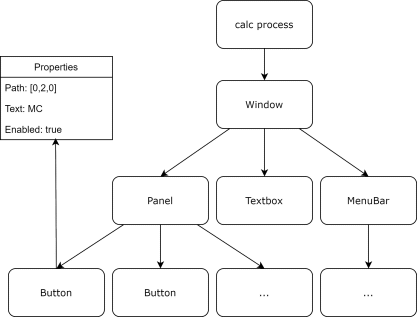
\includegraphics{pics/calc-tree.png}
\captionof{figure}{A compact version of a widget tree for the calculator.}\label{fig:widget-tree}
\endgroup

\subsection{Widget data API}

In order to retrieve data from a SUT, TESTAR is making use of external API's to access widgets that are part of the GUI \cite{thesisMulders}. TESTAR is using three different API's.

In order to test desktop application, TESTAR makes use of the Windows Automation API. The purpose of the Windows Automation API is to expose rich information about UI elements\cite{win-api-info}. For web applications, TESTAR uses Selenium Chromedriver. The Chromedriver is a tool for automated testing. It provides capabilities for navigating through web pages, user input, and JavaScript execution \cite{chrome-driver-info}. The latest API that TESTAR is using is Appinum. Appinum is a test automation tool for native, mobile web, and hybrid applications on iOS mobile, Android mobile, and Windows desktop platforms \cite{apinum-info}

\subsubsection{GUI State} \label{gui-state}

The title of this research proposal is \emph{"\mytitle"}. An inferred model is a directed graph with states and actions. Each vertex represents the application's state. A state is a snapshot of the visible GUI when no action is taking place \cite{gui-history, thesisMulders}. The edges represent actions, for instance, pressing a button. Figure \ref{fig:state-example} shows an example of a graph created for the Windows calculated.

\begingroup
\captionsetup{type=figure}
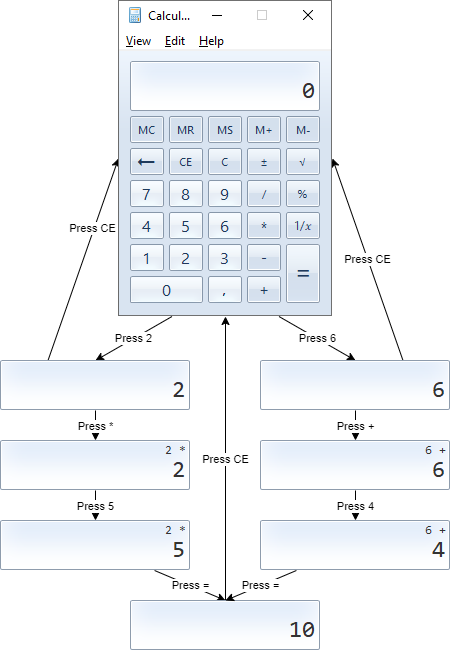
\includegraphics[scale=0.5]{pics/calc-state-example.png}
\captionof{figure}{An example state graph for the Windows Calculator.}\label{fig:state-example}
\endgroup

A directed graph with each vertex a screenshot of the SUT is an example of the \emph{Murphy} tool's output. \emph{Murphy} is developed by a software company from Finland (F-Secure), which can be used to extract GUI models for testing GUI applications automatically. \cite{aho2013industrial}. Although the context for the research is TESTAR, Murphy can be used to research and learn how it detects changes, thus applying that knowledge to TESTAR \cite{murphy-extract-gui}.

To identify the state (and actions), TESTAR calculates two state identifiers; an abstract and concrete state identifier \cite{thesisMulders}. For the concrete state identifier, all the properties of a widget are used. For the abstract identifier, a subset of the properties is used. It is configurable which properties are used for the abstract identifier. By default the properties \textit{role}, \textit{title}, \textit{position} and \textit{enabled} are used.

TESTAR uses the following hashing algorithm: For each widget, the used properties are concatenated and hashed. The hashed widget properties are then joined to create a state hash that identifies it. 

\subsection{How is data persisted}

TESTAR is using a database to store and retrieve state model data. Gier and Kager investigated which data storing solution would be beneficial to TESTAR \cite{GierKager}. The data solution must comply with six requirements. Generally speaking, the requirements were as follows: an open-source graph database with a straightforward query mechanic. The conclusion was that OrientDB was the best solution that met all the requirements.

OrientDB is a Multi-Model NoSQL \acrfull{dbms} that combines four models \cite{orientDbModeling}:

\begin{itemize}
    \item \hyperlink{db:key-value}{Key/Value}
    \item \hyperlink{db:document}{Document}
    \item \hyperlink{db:graph}{Graph}
    \item \hyperlink{db:object}{Object}
\end{itemize}

A \hypertarget{db:key-value}{\emph{Key/Value}} is the simplest model and allows storing information (value) that is accessible with a key. Key/Values can be group into \textit{buckets} however, OrientDB support richer models in the form of document and graph elements.

A \hypertarget{db:document}{\emph{document}} is a schema-less set of key/value pairs. The \emph{key} allows access to the corresponding value. OrientDB allows the developer to store documents into \emph{clusters}. Relations between document are either embedded into other document or \emph{linked} to each other. Someone familiar with relational databases can view a cluster as tables, a document as the row and the key/value pairs are columns.

The \hypertarget{db:graph}{\emph{graph}} is a model consisting of \emph{Vertices} and \emph{Edges}. Vertices are the nodes in the graph, and the edge is the link between those nodes. In TESTAR terminology, a vertex represents state, and the edge is an 'action' from one state to the next. A Vertex consists of three elements: a unique identifier, a set with incoming Edges and outgoing Edges. An edge consists of four elements: a unique identifier, an incoming vertex (\emph{head}), an outgoing vertex (\emph{tail}) and a label that describes the relationship between the head and tail vertex.\par

The last model is the \hypertarget{db:object}{\emph{object}}, which supports inheritance like in the Object-Oriented programming paradigm.\par

Despite being a NoSQL database, OrientDB does support SQL as a query language \cite{sql-lang} albeit that it does not support all SQL statements. The majority of developers have experience with SQL \cite{sql-stats} as a result, new developers and students can start querying the TESTAR data and start expanding its features.\par

In addition to TESTAR, other applications can query the state model data in the OrientDB database as well. For example, developers and students can create external tools for a single purpose, like a state model difference application. When building external tools, the TESTAR application can be kept small and focus upon one objective: testing GUI applications. 